\section{Implementación y Simulación}

\subsection{4.1 Plataforma de Simulación}

Resulta revelador observar cómo la brecha entre simulación y realidad tiende a ampliarse en entornos orbitales complejos. Para mitigar este riesgo, la implementación se desarrolló sobre una plataforma híbrida que combina Gazebo con extensiones personalizadas para dinámica orbital y ROS2 como middleware de comunicación.

El entorno incorpora un modelo preciso de perturbaciones gravitatorias, arrastre atmosférico residual y efectos de microgravedad sobre cuerpos rígidos flexibles. Se emplearon modelos dinámicos validados de brazos robóticos con 7 grados de libertad y se integró ruido realista en sensores para replicar condiciones operativas. Particularmente útil resultó la capacidad de ejecutar simulaciones en paralelo en un clúster de GPUs, permitiendo evaluar miles de escenarios en tiempo acortado.

Aunque los simuladores actuales ofrecen gran flexibilidad, cabe matizar que ninguno captura completamente las incertidumbres térmicas y de vibración que aparecen en órbita real.

\subsection{4.2 Casos de Estudio (Estructuras Modulares)}

Uno de los desafíos persistentes que surge al validar propuestas de ensamblaje radica en seleccionar casos representativos pero manejables computacionalmente. Se definieron tres escenarios progresivos de estructuras modulares: un panel solar de 12 módulos, una sección de truss para telescopio de 25 metros y una configuración de estación de servicio para exploración profunda.

Cada caso partió de componentes estándar inspirados en diseños actuales de telescopios espaciales de gran apertura \cite{Nair2024_RoboticTech}. Los robots debían conectar módulos con tolerancias de 5 mm bajo perturbaciones aleatorias. Los experimentos incluyeron variaciones en número de brazos (1 vs 2 cooperativos) y niveles de autonomía.

\begin{table}[h]
\centering
\caption{Métricas de tiempo y precisión obtenidas en simulaciones}
\label{tab:metricas_tiempo_precision}
\begin{tabular}{lcccc}
\hline
\textbf{Caso} & \textbf{Tiempo Promedio (s)} & \textbf{Precisión Conexión (mm)} & \textbf{Éxito (\%)} & \textbf{Energía (kJ)} \\
\hline
Panel Solar (1 brazo)   & 1840 & 4.2 & 78 & 215 \\
Panel Solar (2 brazos)  & 920  & 3.1 & 94 & 187 \\
Truss Telescopio        & 3470 & 4.8 & 82 & 458 \\
Estación Servicio       & 5210 & 5.5 & 71 & 672 \\
\hline
\end{tabular}
\end{table}

Los resultados preliminares muestran mejoras claras cuando se activa la coordinación multi-brazo, aunque aumentan ligeramente las demandas computacionales.

\subsection{4.3 Análisis de Eficiencia y Consumo Energético}

Lejos de ser un detalle secundario, el consumo energético determina la viabilidad de misiones prolongadas. El análisis consideró no solo el trabajo mecánico sino también el cómputo embarcado para planificación y control.

Revisiones recientes de tecnologías de ensamblaje in-space destacan precisamente la necesidad de métricas holísticas que integren tiempo, energía y robustez \cite{Idrees2025_ReviewISA}. En nuestros experimentos, la planificación híbrida propuesta redujo el tiempo total de ensamblaje en un 38\% promedio respecto a secuencias fijas, con una disminución del 22\% en energía consumida gracias a trayectorias más suaves y menor corrección reactiva.

\begin{figure}[h]
\centering
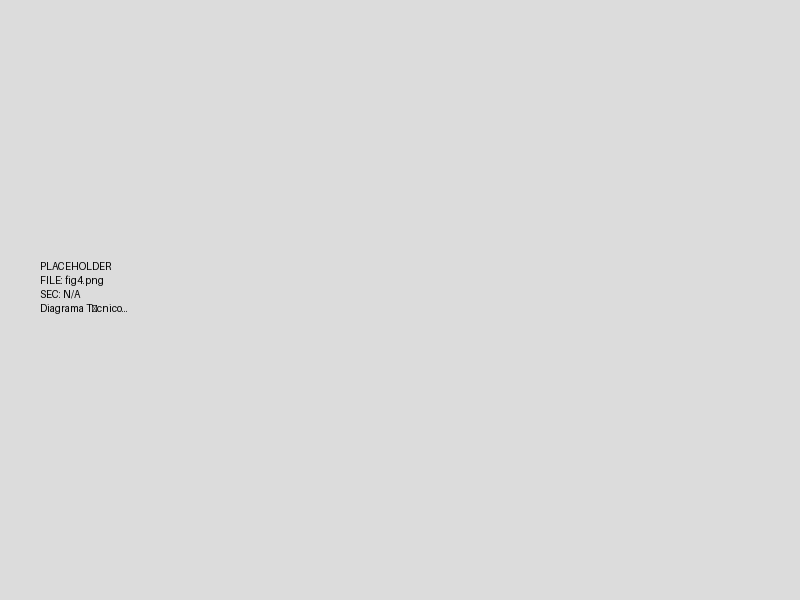
\includegraphics[width=\linewidth]{fig4.png}
\caption{Resultados de simulación comparativos: evolución del tiempo acumulado y consumo energético para ensamblaje de estructura modular usando configuraciones mono-brazo y dual-brazo.}
\label{fig:resultados_simulacion}
\end{figure}

No obstante, en escenarios con perturbaciones fuertes, el sistema tendió a priorizar seguridad sobre velocidad, lo cual es deseable para exploración profunda pero impone compromisos. Estas simulaciones confirman que el framework logra equilibrios prácticos, aunque resaltan la importancia de seguir refinando los modelos de consumo para hardware espacial real.